\documentclass{article}
%
%
\usepackage{geometry}
\geometry{letterpaper, total={6.5in,9in}}
%
%%%%%%%%%%%%%%%%%%%%%%%%%%%%%%%%%%%%%%%%%%%%%
%%              tex2sws                    %%
%%%%%%%%%%%%%%%%%%%%%%%%%%%%%%%%%%%%%%%%%%%%%
%% Defines the environments for sage code
\usepackage{sagetex}
%% Use the  worksheet  boolean to control
%% items like vertical spacing and margins
%% that vary between the printed page and
%% a web page
\usepackage{ifthen}
\newboolean{worksheet}
\ifx \HCode\UnDef \setboolean{worksheet}{false}
\else             \setboolean{worksheet}{true} \fi
%% Use this before any pgf/tikz packages are included
\ifthenelse{\boolean{worksheet}}
{\def\pgfsysdriver{pgfsys-tex4ht.def}}{\relax}
%% Use this if you have hyperlinks
\ifthenelse{\boolean{worksheet}}
{\usepackage[tex4ht]{hyperref}}{\usepackage[pdftex]{hyperref}}
%%%%%%%%%%%%%%%%%%%%%%%%%%%%%%%%%%%%%%%%%%%%%
%%%%%%%%%%%%%%%%%%%%%%%%%%%%%%%%%%%%%%%%%%%%%

\usepackage{tikz}
\usepackage{tkz-graph, tkz-berge}

\title{Circle Graphs}
\author{Robert Beezer}


\begin{document}
%
\maketitle
%
\section{Circle graphs}
%
A graph is \emph{circle graph} if its vertices can be represented as chords of a circle such that two chords interesct if and only if corresponding vertices form an edge in the graph.  As an example of an external link, see the
\href{http://en.wikipedia.org/wiki/Circle_graph}{Wikipedia article}
on circle graphs.  Which is where the tikz code below was lifted from.
%
\section{Incorporating tikz graphics}
%
This is a minor rearrangement of the code for the graphics mentioned in the Wikipedia article.  The effect is to place the two figures side-by-side in a centered table.  The ``scale'' has been reduced to 2 from an original value of 4.
\begin{center}
\begin{tabular}{cc}
  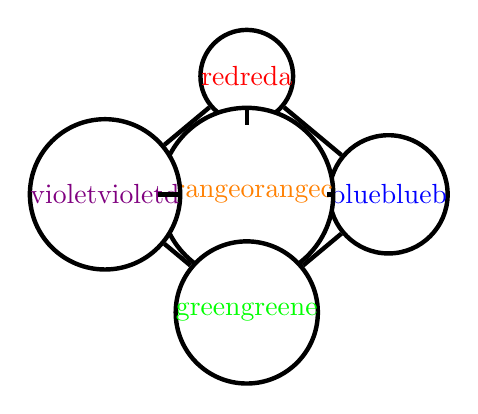
\begin{tikzpicture}[ultra thick,scale=2]
    \foreach \color/\pos/\name in
{{red/(0,-1.5)/a},{blue/(0.9,-2.25)/b},{orange/(0,-2.25)/c},{violet/(-0.9,-2.25)/d},{green/(0,-3)/e}}
      \node[\color,draw,circle,fill=white,minimum size=22pt,inner
sep=0pt] (\name) at \pos {\name};
    \foreach \src/\tgt in {a/b,a/c,a/d,b/c,c/d,b/e,d/e}
      \draw (\src) -- (\tgt);
  \end{tikzpicture}
&
  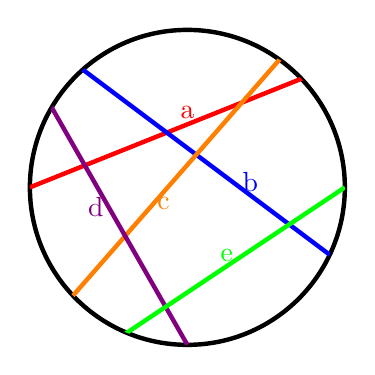
\begin{tikzpicture}[ultra thick,scale=2]
    \clip[draw] (0,0) circle (1cm);
    \draw[red] (-1,0) -- (1,0.8) node[pos=0.5,above=-0.75mm] {a};
    \draw[blue] (-1,1) -- (1,-0.5) node[pos=0.7,above=-1mm] {b};
    \draw[orange] (0.75,1) -- (-1,-1) node[pos=0.55,right=-1mm] {c};
    \draw[violet] (-1,0.75) -- (0,-1) node[midway,left=-0.8mm] {d};
    \draw[green] (-0.5,-1) -- (1,0) node[midway,above=-0.9mm] {e};
  \end{tikzpicture}
\end{tabular}
\end{center}

\section{A small graph generated by Sage}
%
The Heawood graph below was created in Sage, then its latex form was requested, and the output was cut/paste into the source of this document for processing by the tikz-graph package.  It is the unique distance-regular graph $\Gamma$  with intersection array $\left\lbrace 3,2,2;1,1,3\right\rbrace$. It has $14$ vertices and spectrum $3^1\,(\sqrt{2})^6\,(–√2)^6\,(–3)^1$.
See Andries E.\ Brouwer's
\href{http://www.win.tue.nl/~aeb/graphs/Heawood.html}{Heawood Graph Page}
for more information.
\begin{center}
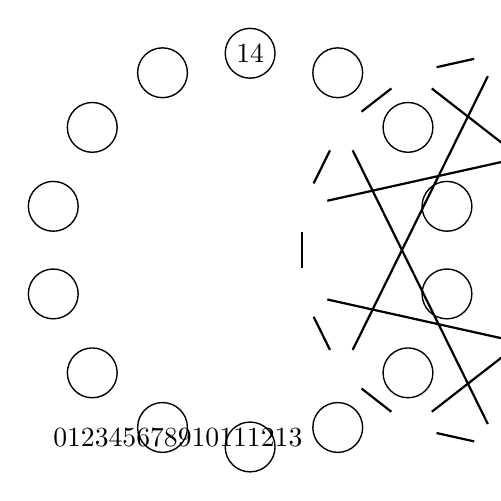
\begin{tikzpicture}
%
\definecolor{col_a0}{rgb}{1.0,1.0,1.0}
\definecolor{col_a1}{rgb}{1.0,1.0,1.0}
\definecolor{col_a2}{rgb}{1.0,1.0,1.0}
\definecolor{col_a3}{rgb}{1.0,1.0,1.0}
\definecolor{col_a4}{rgb}{1.0,1.0,1.0}
\definecolor{col_a5}{rgb}{1.0,1.0,1.0}
\definecolor{col_a6}{rgb}{1.0,1.0,1.0}
\definecolor{col_a7}{rgb}{1.0,1.0,1.0}
\definecolor{col_a8}{rgb}{1.0,1.0,1.0}
\definecolor{col_a9}{rgb}{1.0,1.0,1.0}
\definecolor{col_a10}{rgb}{1.0,1.0,1.0}
\definecolor{col_a11}{rgb}{1.0,1.0,1.0}
\definecolor{col_a12}{rgb}{1.0,1.0,1.0}
\definecolor{col_a13}{rgb}{1.0,1.0,1.0}
%
%
\definecolor{col_lab_a0}{rgb}{0.0,0.0,0.0}
\definecolor{col_lab_a1}{rgb}{0.0,0.0,0.0}
\definecolor{col_lab_a2}{rgb}{0.0,0.0,0.0}
\definecolor{col_lab_a3}{rgb}{0.0,0.0,0.0}
\definecolor{col_lab_a4}{rgb}{0.0,0.0,0.0}
\definecolor{col_lab_a5}{rgb}{0.0,0.0,0.0}
\definecolor{col_lab_a6}{rgb}{0.0,0.0,0.0}
\definecolor{col_lab_a7}{rgb}{0.0,0.0,0.0}
\definecolor{col_lab_a8}{rgb}{0.0,0.0,0.0}
\definecolor{col_lab_a9}{rgb}{0.0,0.0,0.0}
\definecolor{col_lab_a10}{rgb}{0.0,0.0,0.0}
\definecolor{col_lab_a11}{rgb}{0.0,0.0,0.0}
\definecolor{col_lab_a12}{rgb}{0.0,0.0,0.0}
\definecolor{col_lab_a13}{rgb}{0.0,0.0,0.0}
%
%
\definecolor{col_a0-a1}{rgb}{0.0,0.0,0.0}
\definecolor{col_a0-a5}{rgb}{0.0,0.0,0.0}
\definecolor{col_a0-a13}{rgb}{0.0,0.0,0.0}
\definecolor{col_a1-a2}{rgb}{0.0,0.0,0.0}
\definecolor{col_a1-a10}{rgb}{0.0,0.0,0.0}
\definecolor{col_a2-a3}{rgb}{0.0,0.0,0.0}
\definecolor{col_a2-a7}{rgb}{0.0,0.0,0.0}
\definecolor{col_a3-a4}{rgb}{0.0,0.0,0.0}
\definecolor{col_a3-a12}{rgb}{0.0,0.0,0.0}
\definecolor{col_a4-a5}{rgb}{0.0,0.0,0.0}
\definecolor{col_a4-a9}{rgb}{0.0,0.0,0.0}
\definecolor{col_a5-a6}{rgb}{0.0,0.0,0.0}
\definecolor{col_a6-a7}{rgb}{0.0,0.0,0.0}
\definecolor{col_a6-a11}{rgb}{0.0,0.0,0.0}
\definecolor{col_a7-a8}{rgb}{0.0,0.0,0.0}
\definecolor{col_a8-a9}{rgb}{0.0,0.0,0.0}
\definecolor{col_a8-a13}{rgb}{0.0,0.0,0.0}
\definecolor{col_a9-a10}{rgb}{0.0,0.0,0.0}
\definecolor{col_a10-a11}{rgb}{0.0,0.0,0.0}
\definecolor{col_a11-a12}{rgb}{0.0,0.0,0.0}
\definecolor{col_a12-a13}{rgb}{0.0,0.0,0.0}
%
%
\GraphInit[vstyle=Normal]
%
\SetVertexMath
%
\SetVertexNoLabel
%
\renewcommand*{\VertexLightFillColor}{col_a0}
\Vertex[x=2.5cm,y=5.0cm]{a0}
\renewcommand*{\VertexLightFillColor}{col_a1}
\Vertex[x=1.3874cm,y=4.7524cm]{a1}
\renewcommand*{\VertexLightFillColor}{col_a2}
\Vertex[x=0.4952cm,y=4.0587cm]{a2}
\renewcommand*{\VertexLightFillColor}{col_a3}
\Vertex[x=0.0cm,y=3.0563cm]{a3}
\renewcommand*{\VertexLightFillColor}{col_a4}
\Vertex[x=0.0cm,y=1.9437cm]{a4}
\renewcommand*{\VertexLightFillColor}{col_a5}
\Vertex[x=0.4952cm,y=0.9413cm]{a5}
\renewcommand*{\VertexLightFillColor}{col_a6}
\Vertex[x=1.3874cm,y=0.2476cm]{a6}
\renewcommand*{\VertexLightFillColor}{col_a7}
\Vertex[x=2.5cm,y=0.0cm]{a7}
\renewcommand*{\VertexLightFillColor}{col_a8}
\Vertex[x=3.6126cm,y=0.2476cm]{a8}
\renewcommand*{\VertexLightFillColor}{col_a9}
\Vertex[x=4.5048cm,y=0.9413cm]{a9}
\renewcommand*{\VertexLightFillColor}{col_a10}
\Vertex[x=5.0cm,y=1.9437cm]{a10}
\renewcommand*{\VertexLightFillColor}{col_a11}
\Vertex[x=5.0cm,y=3.0563cm]{a11}
\renewcommand*{\VertexLightFillColor}{col_a12}
\Vertex[x=4.5048cm,y=4.0587cm]{a12}
\renewcommand*{\VertexLightFillColor}{col_a13}
\Vertex[x=3.6126cm,y=4.7524cm]{a13}
%
%
\AssignVertexLabel{a}{14}{
\color{col_lab_a0}{$0$},
\color{col_lab_a1}{$1$},
\color{col_lab_a2}{$2$},
\color{col_lab_a3}{$3$},
\color{col_lab_a4}{$4$},
\color{col_lab_a5}{$5$},
\color{col_lab_a6}{$6$},
\color{col_lab_a7}{$7$},
\color{col_lab_a8}{$8$},
\color{col_lab_a9}{$9$},
\color{col_lab_a10}{$10$},
\color{col_lab_a11}{$11$},
\color{col_lab_a12}{$12$},
\color{col_lab_a13}{$13$}
}
%
%
\renewcommand*{\EdgeColor}{col_a0-a1}
\Edge(a0)(a1)
\renewcommand*{\EdgeColor}{col_a0-a5}
\Edge(a0)(a5)
\renewcommand*{\EdgeColor}{col_a0-a13}
\Edge(a0)(a13)
\renewcommand*{\EdgeColor}{col_a1-a2}
\Edge(a1)(a2)
\renewcommand*{\EdgeColor}{col_a1-a10}
\Edge(a1)(a10)
\renewcommand*{\EdgeColor}{col_a2-a3}
\Edge(a2)(a3)
\renewcommand*{\EdgeColor}{col_a2-a7}
\Edge(a2)(a7)
\renewcommand*{\EdgeColor}{col_a3-a4}
\Edge(a3)(a4)
\renewcommand*{\EdgeColor}{col_a3-a12}
\Edge(a3)(a12)
\renewcommand*{\EdgeColor}{col_a4-a5}
\Edge(a4)(a5)
\renewcommand*{\EdgeColor}{col_a4-a9}
\Edge(a4)(a9)
\renewcommand*{\EdgeColor}{col_a5-a6}
\Edge(a5)(a6)
\renewcommand*{\EdgeColor}{col_a6-a7}
\Edge(a6)(a7)
\renewcommand*{\EdgeColor}{col_a6-a11}
\Edge(a6)(a11)
\renewcommand*{\EdgeColor}{col_a7-a8}
\Edge(a7)(a8)
\renewcommand*{\EdgeColor}{col_a8-a9}
\Edge(a8)(a9)
\renewcommand*{\EdgeColor}{col_a8-a13}
\Edge(a8)(a13)
\renewcommand*{\EdgeColor}{col_a9-a10}
\Edge(a9)(a10)
\renewcommand*{\EdgeColor}{col_a10-a11}
\Edge(a10)(a11)
\renewcommand*{\EdgeColor}{col_a11-a12}
\Edge(a11)(a12)
\renewcommand*{\EdgeColor}{col_a12-a13}
\Edge(a12)(a13)
%
%
\end{tikzpicture}
\end{center}


If you would prefer to see Sage's version of this graph, execute the following code block in the worksheet version of this document.
%
\begin{sageverbatim}
G = graphs.HeawoodGraph()
show(G)
\end{sageverbatim}
In the Sage worksheet version of this document, you can rerun the code used to create the latex souce of the tkz-graph version of this graph.

\begin{sageverbatim}
G = graphs.HeawoodGraph()
latex(G)
\end{sageverbatim}

\section{Sage graph editor}

Sage includes a editor that allows you to construct graphs with a point-and-click interface.  The graph below was built this way, then converted to latex and finally pasted into the latex source of this document.

\begin{center}
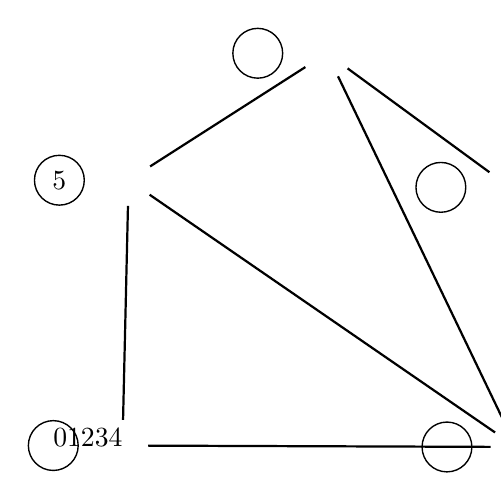
\begin{tikzpicture}
%
\definecolor{col_a0}{rgb}{1.0,1.0,1.0}
\definecolor{col_a1}{rgb}{1.0,1.0,1.0}
\definecolor{col_a2}{rgb}{1.0,1.0,1.0}
\definecolor{col_a3}{rgb}{1.0,1.0,1.0}
\definecolor{col_a4}{rgb}{1.0,1.0,1.0}
%
%
\definecolor{col_lab_a0}{rgb}{0.0,0.0,0.0}
\definecolor{col_lab_a1}{rgb}{0.0,0.0,0.0}
\definecolor{col_lab_a2}{rgb}{0.0,0.0,0.0}
\definecolor{col_lab_a3}{rgb}{0.0,0.0,0.0}
\definecolor{col_lab_a4}{rgb}{0.0,0.0,0.0}
%
%
\definecolor{col_a0-a1}{rgb}{0.0,0.0,0.0}
\definecolor{col_a0-a2}{rgb}{0.0,0.0,0.0}
\definecolor{col_a0-a4}{rgb}{0.0,0.0,0.0}
\definecolor{col_a1-a4}{rgb}{0.0,0.0,0.0}
\definecolor{col_a2-a3}{rgb}{0.0,0.0,0.0}
\definecolor{col_a2-a4}{rgb}{0.0,0.0,0.0}
\definecolor{col_a3-a4}{rgb}{0.0,0.0,0.0}
%
%
\GraphInit[vstyle=Normal]
%
\SetVertexMath
%
\SetVertexNoLabel
%
\renewcommand*{\VertexLightFillColor}{col_a0}
\Vertex[x=0.0775cm,y=3.3877cm]{a0}
\renewcommand*{\VertexLightFillColor}{col_a1}
\Vertex[x=0.0cm,y=0.0181cm]{a1}
\renewcommand*{\VertexLightFillColor}{col_a2}
\Vertex[x=2.5969cm,y=5.0cm]{a2}
\renewcommand*{\VertexLightFillColor}{col_a3}
\Vertex[x=4.9225cm,y=3.2971cm]{a3}
\renewcommand*{\VertexLightFillColor}{col_a4}
\Vertex[x=5.0cm,y=0.0cm]{a4}
%
%
\AssignVertexLabel{a}{5}{
\color{col_lab_a0}{$0$},
\color{col_lab_a1}{$1$},
\color{col_lab_a2}{$2$},
\color{col_lab_a3}{$3$},
\color{col_lab_a4}{$4$}
}
%
%
\renewcommand*{\EdgeColor}{col_a0-a1}
\Edge(a0)(a1)
\renewcommand*{\EdgeColor}{col_a0-a2}
\Edge(a0)(a2)
\renewcommand*{\EdgeColor}{col_a0-a4}
\Edge(a0)(a4)
\renewcommand*{\EdgeColor}{col_a1-a4}
\Edge(a1)(a4)
\renewcommand*{\EdgeColor}{col_a2-a3}
\Edge(a2)(a3)
\renewcommand*{\EdgeColor}{col_a2-a4}
\Edge(a2)(a4)
\renewcommand*{\EdgeColor}{col_a3-a4}
\Edge(a3)(a4)
%
%
\end{tikzpicture}
\end{center}

In the worksheet version of this document, you can experiment with the graph editor.  Construct a graph by clicking to create new vertices.  Then click one vertex to highlight it (it will become red) and then click a second vertex to form an edge from the highlighted vertex to the second vertex.  Use the same process to remove an edge.  Vertices can be deleted by dragging them outside the editing window and dropping them there.\par
%
When you have the editor window available, use the``variable name'' input field to name the graph H.

\begin{sageverbatim}
graph_editor()
\end{sageverbatim}

After saving the graph you can manipulate it with the full range of Sage commands by referencing the graph as H.  For example the commands below will give you basic information about the graph.

\begin{sageverbatim}
print "Number of vertices: ", H.num_verts()
print "Number of edges: ", H.num_edges()
print "Is connected: ", H.is_connected()
\end{sageverbatim}

\end{document}


